%%%%%%%%%%%%%%%%%%%%%%%%%%%%%%%%%%%%%%%%%
% Masters/Doctoral Thesis 
% LaTeX Template
% Version 2.5 (27/8/17)
%
% This template was downloaded from:
% http://www.LaTeXTemplates.com
%
% Version 2.x major modifications by:
% Vel (vel@latextemplates.com)
%
% This template is based on a template by:
% Steve Gunn (http://users.ecs.soton.ac.uk/srg/softwaretools/document/templates/)
% Sunil Patel (http://www.sunilpatel.co.uk/thesis-template/)
%
% Template license:
% CC BY-NC-SA 3.0 (http://creativecommons.org/licenses/by-nc-sa/3.0/)
%
%%%%%%%%%%%%%%%%%%%%%%%%%%%%%%%%%%%%%%%%%

%----------------------------------------------------------------------------------------
%	PACKAGES AND OTHER DOCUMENT CONFIGURATIONS
%----------------------------------------------------------------------------------------

\documentclass[
11pt, % The default document font size, options: 10pt, 11pt, 12pt
%oneside, % Two side (alternating margins) for binding by default, uncomment to switch to one side
english, % ngerman for German
singlespacing, % Single line spacing, alternatives: onehalfspacing or doublespacing
%draft, % Uncomment to enable draft mode (no pictures, no links, overfull hboxes indicated)
%nolistspacing, % If the document is onehalfspacing or doublespacing, uncomment this to set spacing in lists to single
%liststotoc, % Uncomment to add the list of figures/tables/etc to the table of contents
%toctotoc, % Uncomment to add the main table of contents to the table of contents
%parskip, % Uncomment to add space between paragraphs
%nohyperref, % Uncomment to not load the hyperref package
headsepline, % Uncomment to get a line under the header
%chapterinoneline, % Uncomment to place the chapter title next to the number on one line
%consistentlayout, % Uncomment to change the layout of the declaration, abstract and acknowledgements pages to match the default layout
]{MasterThesis} % The class file specifying the document structure

\usepackage[utf8]{inputenc} % Required for inputting international characters
\usepackage[T1]{fontenc} % Output font encoding for international characters
\usepackage{longtable}
\usepackage{listings}
\usepackage{mathpazo} % Use the Palatino font by default
\usepackage{overpic}
\usepackage[backend=biber,style=apa,natbib=true]{biblatex}
\DefineBibliographyStrings{english}{andothers = {\emph{et al}\adddot}}
\usepackage{float}
\usepackage{hyperref}
\addbibresource{references.bib} % The filename of the bibliography
\usepackage{tikz}
\usetikzlibrary{fit,positioning,arrows.meta, backgrounds}

\definecolor{uhhred}{RGB}{144, 74, 77}
\definecolor{uhhred_highlight}{RGB}{226, 0, 26}
\definecolor{ukeblue}{RGB}{105, 146, 187}
\definecolor{ukeblue_highlight}{RGB}{0, 73, 146}
\definecolor{neutralyellow}{RGB}{244, 199, 120}
\usepackage{forest}
\usepackage{multirow}
\usepackage[autostyle=true]{csquotes} % Required to generate language-dependent quotes in the bibliography
\setcounter{secnumdepth}{3}
\setcounter{tocdepth}{3}
\usepackage{xargs}                      % Use more than one optional parameter in a new commands
\usepackage[pdftex,dvipsnames]{xcolor}  % Coloured text etc.
\usepackage{siunitx}
\usepackage[colorinlistoftodos,prependcaption,textsize=tiny]{todonotes}
\newcommandx{\unsure}[2][1=]{\todo[linecolor=red,backgroundcolor=red!25,bordercolor=red,#1]{#2}}
\newcommandx{\change}[2][1=]{\todo[linecolor=blue,backgroundcolor=blue!25,bordercolor=blue,#1]{#2}}
\newcommandx{\info}[2][1=]{\todo[linecolor=OliveGreen,backgroundcolor=OliveGreen!25,bordercolor=OliveGreen,#1]{#2}}
\newcommandx{\improvement}[2][1=]{\todo[linecolor=Plum,backgroundcolor=Plum!25,bordercolor=Plum,#1]{#2}}
\newcommandx{\thiswillnotshow}[2][1=]{\todo[disable,#1]{#2}}
\usepackage[none]{hyphenat}
\emergencystretch=3em
%----------------------------------------------------------------------------------------
%	MARGIN SETTINGS
%----------------------------------------------------------------------------------------
\usepackage[autostyle=true]{csquotes} % Required to generate language-dependent quotes in the bibliography
\geometry{
	paper=a4paper, % Change to letterpaper for US letter
	inner=2.5cm, % Inner margin
	outer=3.8cm, % Outer margin
	bindingoffset=.5cm, % Binding offset
	top=1.5cm, % Top margin
	bottom=1.5cm, % Bottom margin
	%showframe, % Uncomment to show how the type block is set on the page
}
\usepackage{tabularx}
\usepackage{subcaption}
\captionsetup[subfigure]{list=false}

\usepackage[toc, acronym, nonumberlist]{glossaries}
\renewcommand{\glsnamefont}[1]{\textbf{#1}}
\newcommand{\roughly}{\raisebox{0.1ex}{\textasciitilde}}
\providecommand*{\subsubsectionautorefname}{Subsubsection}

\usepackage{subcaption}
% Generate the glossary
\usepackage{datetime}
\usepackage{tikz}
\usetikzlibrary{arrows.meta,positioning,calc}
\makeglossaries
\input{Misc/glossary}
% Methods
% AI

\newacronym{api}{API}{Application Programming Interface}
\newacronym{atp}{ATP}{Adenosintriphosphat}
\newacronym{adp}{ADP}{Adenosindiphosphat}
\newacronym{gdp}{GDP}{Guanosine diphosphate}
\newacronym{bert}{BERT}{Bidirectional Encoder Representations from Transformers}
\newacronym{crims}{CRIMS}{Crystallization Information Management System}
\newacronym{dmasif}{dMaSIF}{differentiable molecular surface interaction fingerprinting}
\newacronym{embl}{EMBL}{\href{https://www.embl.org/sites/hamburg/}{European Molecular Biology Laboratory}}
\newacronym{esm}{ESM}{Evolutionary Scale Model}
\newacronym{pdb}{PDB}{\href{https://www.rcsb.org/}{Protein Data Bank}}
\newacronym{peg}{PEG}{Polyethylene glycol}
\newacronym{pegmme}{PEG-MME}{Polyethylene glycol Monomethyl Ether}
\newacronym{ks}{KS}{Kolmogorov–Smirnov}
\newacronym{sasa}{SASA}{solvent-accessible surface area}
\newacronym{smiles}{SMILES}{Simplified Molecular Input Line Entry System}
\newacronym{ml}{ML}{Machine learning}
\newacronym{mw}{MW}{Molecular weight}
\newacronym{masif}{MaSIF}{molecular surface interaction fingerprinting}
\newacronym{mascl}{MASCL}{Molecular Assembly Simulation in Crystal Lattice}
\newacronym{pi}{pI}{isoelectric point}
\newacronym{asu}{ASU}{asymmetric unit}
\newacronym{prostT5}{ProstT5}{\href{https://github.com/mheinzinger/ProstT5}{Protein structure-sequence T5}}
\newacronym{blast}{Blast}{Basic Local Alignment Search Tool}
\newacronym{uv}{UV}{Ultraviolet}
\newacronym{xgBoost}{XGBoost}{Extreme Gradient Boosting}
\newacronym{hdbscan}{HDBSCAN}{Hierarchical density based clustering}


\newglossaryentry{TPSA}{
    name={TPSA},
    description={Topological polar surface area; sum of polar atom contributions used as a proxy for molecular polarity and hydrogen-bonding capacity}
}

\newglossaryentry{HBD}{
    name={HBD},
    description={Hydrogen bond donors; number of atoms capable of donating a hydrogen bond}
}

\newglossaryentry{HBA}{
    name={HBA},
    description={Hydrogen bond acceptors; number of atoms capable of accepting a hydrogen bond}
}

\newglossaryentry{LogP}{
    name={LogP},
    description={Octanol/water partition coefficient (log scale); measure of molecular hydrophobicity}
}

\newglossaryentry{MR}{
    name={MR},
    description={Molar refractivity; descriptor related to molecular volume and polarizability}
}

\newglossaryentry{RotB}{
    name={RotB},
    description={Number of rotatable bonds; measure of molecular flexibility}
}

\newglossaryentry{FractionCSP3}{
    name={FractionCSP3},
    description={Fraction of carbon atoms in sp\textsuperscript{3} hybridization; indicator of molecular saturation and three-dimensional character}
}

%----------------------------------------------------------------------------------------
%	THESIS INFORMATION
%----------------------------------------------------------------------------------------

\thesistitle{Predicting Protein Crystallization Conditions using Machine Learning} % Your thesis title, this is used in the title and abstract, print it elsewhere with \ttitle
\supervisor{Prof. Dr. Fabian Michael Kern} % Your supervisor's name, this is used in the title page, print it elsewhere with \supname
\examiner{} % Your examiner's name, this is not currently used anywhere in the template, print it elsewhere with \examname
\degree{Master of Science} % Your degree name, this is used in the title page and abstract, print it elsewhere with \degreename
\author{Michael \textsc{Hüppe}, 7785252} % Your name, this is used in the title page and abstract, print it elsewhere with \authorname
\addresses{} % Your address, this is not currently used anywhere in the template, print it elsewhere with \addressname
\newcommand{\aymeltItzen}{\href{https://www.uke.de/allgemein/arztprofile-und-wissenschaftlerprofile/wissenschaftlerprofilseite_aymelt_itzen.html}{ Prof. Dr. Aymelt Itzen }}
\subject{Computer Science} % Your subject area, this is not currently used anywhere in the template, print it elsewhere with \subjectname
\keywords{} % Keywords for your thesis, this is not currently used anywhere in the template, print it elsewhere with \keywordnames
\university{\href{https://www.uni-hamburg.de/}{University of Hamburg}} % Your university's name and URL, this is used in the title page and abstract, print it elsewhere with \univname
\department{\href{https://www.inf.uni-hamburg.de/}{Department of Computer Science}} % Your department's name and URL, this is used in the title page and abstract, print it elsewhere with \deptname
\group{\href{https://www.zbh.uni-hamburg.de/personen/mlbi.html}{Machine Learning in Bioinformatics}} % Your research group's name and URL, this is used in the title page, print it elsewhere with \groupname
\faculty{\href{http://faculty.university.com}{Faculty Name}} % Your faculty's name and URL, this is used in the title page and abstract, print it elsewhere with \facname

\AtBeginDocument{
\hypersetup{pdftitle=\ttitle} % Set the PDF's title to your title
\hypersetup{pdfauthor=\authorname} % Set the PDF's author to your name
\hypersetup{pdfkeywords=\keywordnames} % Set the PDF's keywords to your keywords
}

\begin{document}

\frontmatter % Use roman page numbering style (i, ii, iii, iv...) for the pre-content pages

\pagestyle{plain} % Default to the plain heading style until the thesis style is called for the body content

%----------------------------------------------------------------------------------------
%	TITLE PAGE
%----------------------------------------------------------------------------------------

\begin{titlepage}
\begin{center}

\vspace*{.06\textheight}
{\scshape\LARGE \univname\par}\vspace{1.5cm} % University name
\textsc{\Large Master Thesis}\\[0.5cm] % Thesis type

\HRule \\[0.4cm] % Horizontal line
{\huge \bfseries \ttitle\par}\vspace{0.4cm} % Thesis title
\HRule \\[1.5cm] % Horizontal line
 
\begin{minipage}[t]{0.4\textwidth}
\begin{flushleft} \large
\emph{Author:}\\
\href{https://www.linkedin.com/in/michael-h\%C3\%BCppe-1053b61a1/?originalSubdomain=de}{\authorname} % Author name - remove the \href bracket to remove the link
\end{flushleft}
\end{minipage}
\begin{minipage}[t]{0.4\textwidth}
\begin{flushright} \large
\emph{Supervisors:} \\
\href{https://www.zbh.uni-hamburg.de/personen/mlbi/fkern.html}{\supname} % Supervisor name - remove the \href
\newline
\aymeltItzen
\end{flushright}
\end{minipage}\\[3cm]
 
\vfill

\large \textit{A thesis submitted in fulfillment of the requirements\\ for the degree of \degreename}\\[0.3cm] % University requirement text
\textit{in the}\\[0.4cm]
MIN-Faculty \\\deptname\\ Computer Science \\ [2cm] % Research group name and department name
 
\vfill

{\large \today}\\[4cm] % Date
%\includegraphics{Logo} % University/department logo - uncomment to place it
 
\vfill
\end{center}
\end{titlepage}

%----------------------------------------------------------------------------------------
%	DECLARATION PAGE
%----------------------------------------------------------------------------------------

\begin{declaration}
\addchaptertocentry{\authorshipname} % Add the declaration to the table of contents
Hiermit versichere ich an Eides statt, dass ich die vorliegende Arbeit im Masterstudiengang Informatik
selbstständig verfasst und keine anderen als die angegebenen Hilfsmittel –- insbesondere keine im Quellenverzeichnis nicht benannten Internet-Quellen –- benutzt habe. Alle Stellen, die wörtlich oder sinngemäß aus Veröffentlichungen entnommen wurden, sind als solche kenntlich gemacht. Ich versichere weiterhin, dass ich die Arbeit vorher nicht in einem anderen Prüfungsverfahren eingereicht habe. Sofern im Zuge der Erstellung der vorliegenden Abschlussarbeit generative Künstliche Intelligenz (gKI) basierte elektronische Hilfsmittel verwendet wurden, versichere ich, dass meine eigene Leistung im Vordergrund stand und dass eine vollständige Dokumentation aller verwendeten Hilfsmittel gemäß der Guten Wissenschaftlichen Praxis vorliegt. Ich trage die Verantwortung für eventuell durch die gKI generierte fehlerhafte oder verzerrte Inhalte, fehlerhafte Referenzen, Verstöße gegen das Datenschutz- und Urheberrecht oder Plagiate. 
\vspace{1cm}


\noindent Signed:\\
\rule[0.5em]{25em}{0.5pt} % This prints a line for the signature
 
\noindent Date:\\
\rule[0.5em]{25em}{0.5pt} % This prints a line to write the date
\end{declaration}

\cleardoublepage

%----------------------------------------------------------------------------------------
%	ABSTRACT PAGE
%----------------------------------------------------------------------------------------

\begin{abstract}
\addchaptertocentry{\abstractname} % Add the abstract to the table of contents
Protein crystallization remains a critical bottleneck in structural biology, as identifying suitable crystallization conditions is largely empirical, time-consuming, and associated with high failure rates. While recent advances in protein structure prediction have significantly improved access to structural information, they do not eliminate the need for experimentally determined crystal structures. This thesis investigates whether machine learning can be used to predict protein crystallization conditions directly from protein-derived features, thereby reducing the experimental search space.

To address this problem, a large-scale dataset was constructed from the \gls{pdb}, comprising nearly 200,000 protein structures along with their associated crystallization metadata. A comprehensive data processing pipeline was developed to transform heterogeneous and partially incomplete experimental records into a structured, machine-readable representation of crystallization conditions. Multiple feature modalities were explored, including sequence-based descriptors, learned sequence embeddings, structural information, and surface-derived properties.

Given the scarcity of reliable negative labels in crystallization data, this work adopts a contrastive learning framework to model the relationship between proteins and crystallization conditions. By using this approach the task is reformulated from crystallization condition prediction to a ranking problem over a discrete condition space. A two-module architecture is proposed, where protein and condition representations are learned jointly in a shared embedding space and compared using a similarity-based scoring function. 

Sequence similarity based splitting and the scoring of past experimental results demonstrate that the proposed approach captures meaningful relationships between protein features and crystallization conditions. This enables the ranking of candidate conditions for an unseen protein. While exact prediction of optimal conditions remains challenging due to the high dimensionality and difficulty of crystallization, the model shows potential to narrow down the experimental search space by 65\% while still capturing 71\% of crystal conditions.

Overall, this work highlights the feasibility of leveraging machine learning for condition prediction in protein crystallization and provides a foundation for future research integrating structural, physicochemical, and experimental data to guide crystallization experiments more efficiently.
\end{abstract}

\begin{acknowledgements}
\addchaptertocentry{\acknowledgementname}
I would like to express my heartfelt gratitude to the individuals who have contributed to the successful completion of this thesis.\\
First and foremost, I would like to extend my appreciation to Dr. Michael Hecht-Bucher.  His support, guidance, and expertise in the fields of structural biology and bioinformatics have been instrumental throughout the entire process. His mentorship has greatly enhanced the quality of my work and understanding of the topics covered.\\
I am also grateful to Prof. Dr. Fabian Kern, for the support in machine learning and bioinformatics and his supervision in this thesis. \\
Moreover, I would like to thank Prof. Dr. Aymelt Itzen for welcoming me into his research group despite my background in a different field, for providing access to laboratory-generated data, and for sharing his expertise in structural biology. \\
A special note of appreciation goes to the Itzen Lab in general for welcoming me into the group and their help in tracking down their crystallization data of past years. Their involvement and cooperation have made the assumptions about real life practicality of the system possible, and their voluntary contribution is sincerely appreciated.\\
Lastly, I would like to extend a huge thank you to my family and friends for their support. \\
My sincere thanks to all of the above for being a part of this thesis and making this a truly rewarding learning experience.\\

\end{acknowledgements}


%----------------------------------------------------------------------------------------
%	LIST OF CONTENTS/FIGURES/TABLES PAGES
%----------------------------------------------------------------------------------------

\tableofcontents % Prints the main table of contents

\listoffigures % Prints the list of figures

\listoftables % Prints the list of tables

\setglossarystyle{long}
\printglossary[type=\acronymtype,title={List of Acronyms}]
%----------------------------------------------------------------------------------------
%	ABBREVIATIONS
%----------------------------------------------------------------------------------------

%----------------------------------------------------------------------------------------
%	DEDICATION
%----------------------------------------------------------------------------------------

%----------------------------------------------------------------------------------------
%	THESIS CONTENT - CHAPTERS
%----------------------------------------------------------------------------------------

\mainmatter % Begin numeric (1,2,3...) page numbering

\pagestyle{thesis} % Return the page headers back to the "thesis" style

% Include the chapters of the thesis as separate files from the Chapters folder
% Uncomment the lines as you write the chapters


\include{Chapters/Introduction}
\include{Chapters/Data}
\chapter{Methods}\label{methods}

\input{Chapters/Methods/features.tex}

\section{Model Architecture}
\label{sec:methods/model_architecture}
\begin{figure}[h]
\centering
\resizebox{\textwidth}{!}{
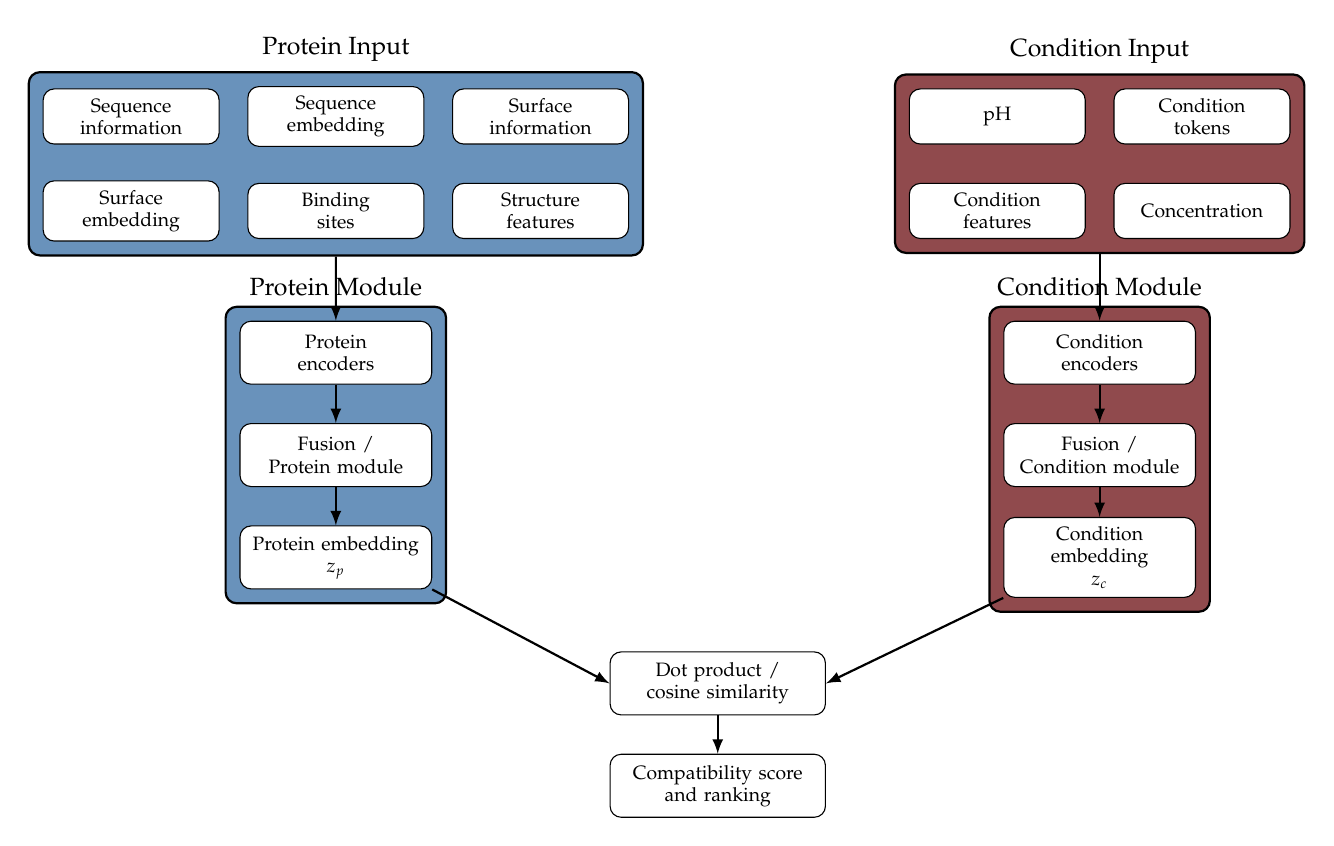
\begin{tikzpicture}[
    font=\scriptsize,
    >=latex,
    box/.style={draw, rounded corners, align=center, text width=2.2cm, minimum height=0.8cm, fill=white},
    smallbox/.style={draw, rounded corners, align=center, text width=2.0cm, minimum height=0.7cm, fill=white},
    group/.style={draw, rounded corners, thick, inner sep=5pt, fill=uhhred},
    groupProtein/.style={draw, rounded corners, thick, inner sep=5pt, fill=ukeblue},
    moduleboxProtein/.style={draw, rounded corners, thick, fill=ukeblue, inner sep=5pt},
    moduleboxCondition/.style={draw, rounded corners, thick, fill=uhhred, inner sep=5pt},
    arrow/.style={->, thick}
]

% ===================== PROTEIN INPUT =====================
\node[smallbox] (seqinfo) at (0,0) {Sequence\\information};
\node[smallbox] (seqemb) at (2.6,0) {Sequence\\embedding};
\node[smallbox] (surfinfo) at (5.2,0) {Surface\\information};

\node[smallbox] (surfemb) at (0,-1.2) {Surface\\embedding};
\node[smallbox] (bind) at (2.6,-1.2) {Binding\\sites};
\node[smallbox] (structfeat) at (5.2,-1.2) {Structure\\features};

% ===================== PROTEIN TOWER =====================
\node[box] (protenc) at (2.6,-3.0) {Protein\\encoders};
\node[box] (protfuse) at (2.6,-4.3) {Fusion /\\Protein module};
\node[box] (protemb) at (2.6,-5.6) {Protein embedding\\$z_p$};

% ===================== CONDITION INPUT =====================
\node[smallbox] (ph) at (11,0) {pH};
\node[smallbox] (tokens) at (13.6,0) {Condition\\tokens};
\node[smallbox] (condfeat) at (11,-1.2) {Condition\\features};
\node[smallbox] (conc) at (13.6,-1.2) {Concentration};

% ===================== CONDITION TOWER =====================
\node[box] (condenc) at (12.3,-3.0) {Condition\\encoders};
\node[box] (condfuse) at (12.3,-4.3) {Fusion /\\Condition module};
\node[box] (condemb) at (12.3,-5.6) {Condition embedding\\$z_c$};

% ===================== SCORING =====================
\node[box, text width=2.5cm] (score) at (7.45,-7.2)
{Dot product /\\cosine similarity};

\node[box, text width=2.5cm] (rank) at (7.45,-8.5)
{Compatibility score\\and ranking};

% ===================== BACKGROUND =====================
\begin{pgfonlayer}{background}
\node[groupProtein, fit=(seqinfo)(seqemb)(surfinfo)(surfemb)(bind)(structfeat),
      label={[font=\small]above:Protein Input}] (proteinin) {};

\node[moduleboxProtein, fit=(protenc)(protfuse)(protemb),
      label={[font=\small]above:Protein Module}] (proteinmodule) {};

\node[group, fit=(ph)(tokens)(condfeat)(conc),
      label={[font=\small]above:Condition Input}] (condin) {};

\node[moduleboxCondition, fit=(condenc)(condfuse)(condemb),
      label={[font=\small]above:Condition Module}] (conditionmodule) {};
\end{pgfonlayer}

% ===================== ARROWS =====================
\draw[arrow] (proteinin.south) -- (protenc.north);
\draw[arrow] (protenc) -- (protfuse);
\draw[arrow] (protfuse) -- (protemb);

\draw[arrow] (condin.south) -- (condenc.north);
\draw[arrow] (condenc) -- (condfuse);
\draw[arrow] (condfuse) -- (condemb);

\draw[arrow] (protemb.south east) -- (score.west);
\draw[arrow] (condemb.south west) -- (score.east);
\draw[arrow] (score) -- (rank);

\end{tikzpicture}
}
\caption[Simplified overview of the two-module architecture]{Simplified overview of the proposed two-module architecture. Protein-related inputs are grouped and passed through the protein module, while condition-related inputs are grouped and passed through the condition module. The resulting embeddings are compared using a similarity-based scoring function to rank candidate conditions.}
\label{fig:model_architecture}
\end{figure}

The proposed model follows a \emph{two-module ranking architecture} in which proteins and crystallization conditions are encoded separately into a shared latent space. The final compatibility score is computed as the dot product between the normalized protein and condition embeddings. This design is well suited for retrieval and ranking tasks because both sides can be embedded independently and compared efficiently.

The architecture is designed around three principles. First, it handles \emph{heterogeneous multimodal inputs} by assigning each modality a dedicated encoder. Second, it uses \emph{late fusion} through separate modules, which keeps the representation learning for proteins and conditions modular and scalable. Third, the normalized shared embedding space provides a natural basis for \emph{retrieval and ranking}, which is particularly useful when many candidate conditions must be evaluated for each protein.

An important advantage of this design is that domain-specific features, pretrained embeddings, and set-structured inputs such as surface points or token lists can be combined in a unified framework. At the same time, the two-module formulation keeps inference efficient because protein and condition representations do not need to be recomputed jointly for every pair.

The overarching model can be described as follows:
Let $x_p$ denote the protein input and $x_c$ the condition input. The model learns two functions
\begin{equation}
    f_p(x_p) \in \mathbb{R}^{d_t}, \qquad f_c(x_c) \in \mathbb{R}^{d_t},
\end{equation}
where $d_t$ is the module dimension. Both outputs are $\ell_2$-normalized:
\begin{equation}
    \hat{z}_p = \frac{f_p(x_p)}{\|f_p(x_p)\|_2}, \qquad
    \hat{z}_c = \frac{f_c(x_c)}{\|f_c(x_c)\|_2}.
\end{equation}
The final score is then
\begin{equation}
    s(x_p, x_c) = \hat{z}_p^\top \hat{z}_c,
\end{equation}
which corresponds to the cosine similarity between the two embeddings. High scores indicate that a condition is predicted to be compatible with a protein.

\subsection{Protein Module}

The protein module integrates feature branches for every feature type presented in \autoref{sec:methods/feature_engineering}.
Each modality is first processed by its own branch-specific encoder. For low-dimensional tabular inputs, the model uses a \gls{mlp}. For high-dimensional pretrained embeddings, a separate head MLP with dropout is used. If enabled, layer normalization is applied before these heads.

Formally, if the active protein branches produce vectors
\begin{equation}
    h^{(1)}_p, h^{(2)}_p, \dots, h^{(m)}_p,
\end{equation}
they are concatenated into one joint representation
\begin{equation}
    h_p = \mathrm{concat}\!\left(h^{(1)}_p, h^{(2)}_p, \dots, h^{(m)}_p\right).
\end{equation}
This concatenated vector is passed through a shared protein module:
\begin{equation}
    z_p = W_{p,2} \, \phi\!\left(\mathrm{LN}\!\left(W_{p,1} h_p + b_{p,1}\right)\right) + b_{p,2},
\end{equation}
where $\phi(\cdot)$ denotes the GELU activation, $\mathrm{LN}$ denotes layer normalization, and dropout is applied after the first hidden transformation. The output $z_p$ is finally normalized to unit length. Each of these feature branches is encoded independently by an MLP or head MLP before fusion into the protein module.

\subsection{Condition Module}

The condition module combines pH, chemical condition tokens, condition-level numerical features, and concentration information. Its purpose is to transform a heterogeneous description of a crystallization condition into a dense representation in the same latent space as the protein module.
The chemical condition encoder combines three sources of information. As described in \autoref{sec:methods/feature_engineering/condition_embedding}, a dense numerical condition features and Morgan fingerprints. Additionally, the pH, concentration and tokens of the chemicals.
Each token represents a unique chemical. Each condition may contain a variable-length list of tokens. These are embedded via a learnable embedding table:
\begin{equation}
    e_i = E[t_i],
\end{equation}
where $t_i$ is the $i$-th token and $E$ is the token embedding matrix. The embedded tokens are further transformed with a residual MLP. Because token sequences have variable length, padded elements are masked and the token representation is obtained using a masked mean:
\begin{equation}
    h_{\text{tok}} =
    \frac{\sum_{i=1}^{T} m_i \tilde{e}_i}{\sum_{i=1}^{T} m_i},
\end{equation}
where $m_i \in \{0,1\}$ indicates whether a token is valid. This prevents padding from influencing the pooled representation.
The numerical condition vector, the pH as well as the concentration are all encoded by an associated \gls{mlp} and concatenated and mapped to the final chemical condition vector through a fusion MLP.
The pH embedding and chemical condition embedding are also concatenated and projected by the condition module.
As in the protein module, the output is finally normalized.

\paragraph{Generic MLP Blocks}

A central component of the architecture is a configurable MLP block used throughout the model. Given an input $x$, an MLP applies a sequence of affine transformations, optional layer normalization, a non-linear activation, and optional dropout:
\begin{equation}
    h^{(l+1)} = \mathrm{Dropout}\!\left(\phi\!\left(\mathrm{LN}(W^{(l)} h^{(l)} + b^{(l)})\right)\right).
\end{equation}
The implementation supports ReLU, GELU, and SiLU activations. Some branches optionally use residual connections:
\begin{equation}
    y = \mathrm{MLP}(x) + x,
\end{equation}
which helps preserve information and stabilize optimization when input and output dimensions are equal.

\paragraph{Scoring Function and Ranking Interpretation}

After obtaining the normalized protein and condition representations, the model computes a single scalar compatibility score using the dot product:
\begin{equation}
    s = \hat{z}_p^\top \hat{z}_c.
\end{equation}
Because both embeddings are normalized, this score lies in the cosine-similarity space. The model can therefore be interpreted as a ranking model: for a fixed protein, multiple candidate conditions can be embedded independently and ranked by decreasing score. Likewise, condition embeddings can be precomputed and reused efficiently during inference.


\section{Data split}
Neither the \gls{pdb} nor the \gls{crims} dataset can be split into training and validation sets using a simple random split. Two main characteristics of these datasets make such an approach inappropriate. The following describes the employed informed split strategy to avoid data leakage to enable a confident report in generalization performance.

First, the \gls{pdb} is highly redundant. The same protein is often deposited multiple times in the database, for example with different resolutions, slightly modified constructs, ligand bindings, or other experimental variations. At the time the data for this thesis was collected, the \gls{pdb} contained approximately 197,000 structure entries, but these corresponded to only about 89,000 unique proteins. Some proteins appear extremely frequently. For instance, the proteins R1AB\_SARS2 and LYSC\_CHICK had 2631 and 1258 associated structure files respectively. This is further depicted in \autoref{fig:most_common_proteins} in \autoref-{app:data}.


This redundancy has important implications for machine learning. As shown in \autoref{fig:proteinVsPEGComparison}, proteins tend to be highly selective with respect to their crystallization conditions. This selectivity arises from two main factors. First, the same protein often crystallizes reproducibly under similar conditions due to its structural and physicochemical properties. Second, once a successful crystallization condition has been reported in the \gls{pdb}, subsequent experiments frequently begin their condition search near previously successful conditions. This creates a strong bias linking specific proteins to specific crystallization conditions.

Although the protein name or identifier is not explicitly included as an input feature, the model can still indirectly learn protein identity through the protein sequence embedding. As illustrated in \autoref{fig:proteinEmbedding}, proteins form strong clusters in embedding space, indicating that the model could easily memorize protein-specific condition relationships. If a random split were used, it would therefore be very likely that the same protein—or even the same protein–condition pair—would appear in both the training and validation sets. Such data leakage would lead to overly optimistic performance estimates, as the model could simply recall previously seen patterns rather than learning generalizable relationships.

Avoiding leakage by splitting only by protein identity is insufficient. Although the determinants of crystallization conditions are not fully understood, properties such as structure, surface chemistry, and charge distribution strongly influence crystal formation \citep{Nanev2018}. These properties are implicitly encoded in the amino acid sequence, meaning similar sequences may lead to similar crystallization behavior. Thus, if related proteins appear in both training and validation sets, indirect leakage via sequence similarity can occur.

However, this assumption is debated. Studies such as \citet{Abrahams2019} and \citet{Liao2025} show that similar sequences can exhibit substantially different crystallization behavior, indicating that sequence similarity alone is not a reliable predictor. Nevertheless, to ensure rigorous validation and minimize potential leakage, sequence-based clustering is used when constructing data splits.

To address this issue, an additional level of separation based on sequence similarity clustering is required. A common strategy is to cluster proteins according to their sequence similarity and then ensure that proteins from the same cluster are assigned exclusively to either the training or the validation set. This ensures that the model cannot rely on closely related homologous proteins when making predictions.

For this purpose, sequence similarity clusters generated with MMseqs2 were used. Both the \gls{pdb} and \gls{crims} proteins were clustered at multiple sequence identity thresholds: 30, 40, 50, 70, 90, 95, and 100\% sequence identity. The clustering was performed using the easy-cluster algorithm of MMseqs2, which efficiently groups sequences into clusters based on pairwise sequence similarity. In this procedure, sequences are compared using fast k-mer based prefiltering followed by sequence alignment. Proteins are assigned to the same cluster if their sequence identity exceeds the specified threshold while satisfying coverage constraints (here using parameters c=0.8, cov-mode=0, and identity threshold ID=N). This ensures that sequences within a cluster share a minimum level of alignment coverage and sequence identity.

Lower identity thresholds produce broader clusters that group together more distantly related proteins, while higher thresholds result in tighter clusters containing only very similar or nearly identical sequences. Consequently, the 30\% identity clustering represents the most challenging evaluation scenario, as proteins in the validation set share only weak homology with proteins seen during training. In contrast, the 100\% identity clustering is the most permissive setting, where proteins in the validation set may be nearly identical to those present in the training set.

From an inference perspective, these splits correspond to different assumptions about the model's applicability. If the model performs well on the 30\% sequence identity split, it suggests that the model can infer crystallization conditions for proteins even when no closely related homologs are present in the training data. This would indicate strong generalization capability. On the other hand, strong performance on the 100\% identity split only demonstrates that the model can reproduce crystallization conditions for proteins that are essentially identical to proteins already present in the training set.

Evaluating the model across multiple sequence identity thresholds therefore provides a more comprehensive understanding of its generalization behavior, ranging from near-memorization scenarios to genuinely novel protein prediction tasks. \autoref{fig:train_test_split} depicts a schematic illustration. 


\section{Training}
\subsection{Training Procedure}\label{sec:methods/training}

The model is trained using a contrastive ranking objective within a two-tower architecture. The goal is to learn a shared embedding space in which compatible protein--condition pairs have high similarity, while incompatible pairs are separated.
Each training batch consists of $B$ paired samples:
\begin{equation}
    \{(x_p^{(i)}, x_c^{(i)})\}_{i=1}^{B},
\end{equation}
where $x_p^{(i)}$ denotes the protein features and $x_c^{(i)}$ the corresponding crystallization condition. Each condition is additionally associated with a unique identifier $c^{(i)}$.

As seen in \autoref{fig:mostcommoncocktails} in \autoref{sec:data_analysis} some conditions occure multiple. This means that unlike standard contrastive setups, batches may contain duplicate conditions. Using standard batch contrastive learning the diagonal in a batch is optimized i.e. duplicates in a batch would be turned into false negatives. To accomodate this in the designed setup the duplicates are explicitly leveraged during training by treating all identical conditions as valid positives. This is done by comparing the conditions based on their chemical composition and pH. 
As described in \autoref{sec:methods/model_architecture} for each batch, protein and condition inputs are encoded independently using the two towers:
\begin{equation}
    z_p^{(i)} = f_p(x_p^{(i)}), \qquad
    z_c^{(j)} = f_c(x_c^{(j)}).
\end{equation}

Both embeddings are $\ell_2$-normalized, and a full pairwise similarity matrix is computed:
\begin{equation}
    S_{ij} = \frac{z_p^{(i)}}{\|z_p^{(i)}\|_2}^\top
             \frac{z_c^{(j)}}{\|z_c^{(j)}\|_2}.
\end{equation}

This results in a $B \times B$ score matrix where each row corresponds to a protein and each column to a condition.
On this score matrix a mask is employed to mask-out loss for duplicate conditions. Thus, all conditions in the batch with the same identifier are treated as valid positives for a given protein.

The training objective is based on a multi-positive variant of the InfoNCE loss. For each anchor $i$, the probability assigned to its positives is:
\begin{equation}
    p_{ij} = \frac{\exp(S_{ij} / \tau)}
    {\sum_{k=1}^{B} \exp(S_{ik} / \tau)},
\end{equation}
where $\tau$ is a temperature parameter controlling the sharpness of the distribution.

The row-wise loss (protein-to-condition direction) is defined as:
\begin{equation}
    \mathcal{L}_{\text{row}} =
    - \frac{1}{B} \sum_{i=1}^{B}
    \frac{1}{|P(i)|}
    \sum_{j \in P(i)} \log p_{ij},
\end{equation}
where $P(i)$ denotes the set of positive indices for anchor $i$.

Similarly, a column-wise loss (condition-to-protein direction) is computed:
\begin{equation}
    \mathcal{L}_{\text{col}} =
    - \frac{1}{B} \sum_{j=1}^{B}
    \frac{1}{|Q(j)|}
    \sum_{i \in Q(j)} \log p_{ij},
\end{equation}
where $Q(j)$ denotes all proteins associated with condition $j$.

The final symmetric loss is a weighted combination:
\begin{equation}
    \mathcal{L}_{\text{rank}} =
    (1 - \lambda)\, \mathcal{L}_{\text{row}} +
    \lambda\, \mathcal{L}_{\text{col}},
\end{equation}
where $\lambda \in [0,1]$ controls the relative importance of both directions.

This symmetric formulation ensures that 1. proteins retrieve all compatible conditions and 2. conditions retrieve all associated proteins.
In addition to the ranking loss, an auxiliary contrastive regularization term is applied to the protein embeddings. 

All non-positive pairs within a batch are implicitly treated as negatives. This yields $O(B^2)$ training pairs without additional sampling. The effectiveness of this approach depends on sufficiently large and diverse batches.
In addition to loss and performance metrics, gradient norms of individual model components are monitored to ensure stable optimization across different branches of the architecture.
At inference time, protein and condition embeddings can be computed independently. Given a protein embedding $z_p$, candidate conditions $\{z_c^{(j)}\}$ are ranked according to:
\begin{equation}
    s_j = z_p^\top z_c^{(j)}.
\end{equation}
This enables efficient retrieval of suitable crystallization conditions from large candidate sets.

\subsection{Evaluation Metrics}

The central challenge in macromolecular crystallography is the large number of experiments that must typically be performed in order to identify a suitable crystallization condition. Because laboratory experiments are costly and time-consuming, reducing the number of required trials is the main objective in this thesis.

A straightforward formulation of this task would be to predict the optimal crystallization condition directly for a given protein. While such an approach would be highly valuable in practice, it is also extremely challenging. A single protein can crystallize under a wide variety of chemically distinct conditions involving different buffers, salts, precipitants, and pH values \citep{Liao2025}. Consequently, it is often difficult to define a single optimal condition.

In practice, crystallographers frequently report only one successful crystallization condition to the \gls{pdb}, often selecting the condition that is easiest to reproduce experimentally. As a result, the \gls{pdb} contains only positive crystallization outcomes and lacks explicit negative examples. In contrast, experimental screening data, such as the \gls{crims} dataset described in \autoref{sec:crims}, contains numerous unsuccessful trials. As illustrated in \autoref{fig:crims_categorical_analysis}, the vast majority of experiments do not lead to crystal formation, resulting in a highly imbalanced dataset with far more negative than positive observations.

This imbalance has important implications for both model design and evaluation. The task can be reformulated as a binary classification problem: given a protein and a candidate crystallization condition, the model predicts whether the experiment is likely to produce a crystal. Because successful crystallization events are rare, standard evaluation metrics such as overall accuracy can provide misleading assessments of model performance. A classifier that simply predicts failure for every condition would achieve high accuracy while being practically useless.

Evaluation metrics that account for class imbalance and emphasize the detection of positive outcomes are particularly important. In the context of crystallization screening, missing a potentially successful condition (a false negative) is more detrimental than testing a condition that ultimately fails (a false positive). Similar to the image classification model presented in \autoref{sec:crims/confirmation_protein_crystals} a sensitivity is more valuable than sensibility. Therefore, metrics that measure the ability of the model to correctly identify positive outcomes, such as positive recall, are of special interest.

In the following, the metrics and visualizations used to evaluate the binary classification models are described.

\paragraph{Confusion Matrix}
The confusion matrix provides a comprehensive overview of the predictions made by a binary classifier. It summarizes the number of correctly and incorrectly classified samples in four categories:

\begin{itemize}
	\itemsep0em
    \item \gls{tp}: successful crystallization conditions correctly predicted as successful.
    \item \gls{fn}: unsuccessful conditions incorrectly predicted as successful.
    \item \gls{tn}: unsuccessful conditions correctly predicted as unsuccessful.
    \item \gls{fp}: successful conditions incorrectly predicted as unsuccessful.
\end{itemize}

From these quantities, several informative performance metrics can be derived. In the context of crystallization prediction, false negatives are particularly undesirable because they correspond to potentially viable crystallization conditions that would be discarded by the model.

\paragraph{Recall (Sensitivity)}
Recall, also referred to as the \gls{tpr} or sensitivity, measures the proportion of actual positive samples that are correctly identified:

\begin{equation}
\text{Recall} = \frac{TP}{TP + FN}.
\end{equation}

A high positive recall indicates that the model successfully identifies most of the conditions that lead to crystal formation. 

\paragraph{Accuracy}
Accuracy measures the proportion of correctly classified samples:

\begin{equation}
\text{Accuracy} = \frac{TP + TN}{TP + TN + FP + FN}.
\end{equation}

While accuracy is widely used, it is not well suited for strongly imbalanced datasets.

\paragraph{Balanced Accuracy}
Balanced accuracy addresses the limitation of a highly biased model by computing the average recall across both classes using the \gls{tpr} and the \gls{tnr}:

\begin{equation}
\text{Balanced Accuracy} = \frac{\text{TPR} + \text{TNR}}{2}.
\end{equation}

This metric ensures that performance on both classes contributes equally to the final score and therefore provides a more informative evaluation in the presence of class imbalance.

\paragraph{Precision}
Precision quantifies how many predicted positive samples are actually correct:

\begin{equation}
\text{Precision} = \frac{TP}{TP + FP}.
\end{equation}

High precision indicates that predicted successful crystallization conditions are reliable, reducing the number of unnecessary experiments that are expected to fail.

\paragraph{F1 Score}
The F1 score combines precision and recall into a single metric by computing their harmonic mean:

\begin{equation}
F_1 = 2 \cdot \frac{\text{Precision} \cdot \text{Recall}}{\text{Precision} + \text{Recall}}.
\end{equation}

Macro-averaged and weighted variants of the F1 score are used to account for class imbalance and provide a more balanced view of model performance across both classes.

\paragraph{Threshold Analysis}
The models used in this work output probabilities that indicate how likely a given crystallization condition is to produce a crystal. To convert these probabilities into binary predictions, a decision threshold must be chosen.

Different thresholds result in different trade-offs between detecting successful crystallization conditions and avoiding false positives. To analyze this behavior, model performance was evaluated across a range of thresholds. In particular, the positive recall, \gls{tnr} (specificity), and balanced accuracy were plotted as functions of the decision threshold. This analysis allows the identification of thresholds that provide a desirable balance between discovering potential crystallization conditions and limiting unnecessary experiments.

\paragraph{Recall–Specificity Trade-off}
To further illustrate the trade-off between detecting successful crystallization conditions and rejecting unsuccessful ones, recall was plotted against the \gls{tnr} across varying thresholds. This visualization highlights how increasing sensitivity to positive outcomes typically reduces specificity, and vice versa. Such analyzes provide insight into how the model can be tuned depending on whether the experimental objective prioritizes discovering as many potential crystallization conditions as possible or minimizing the number of failed experiments.
\subsection{Hyperparameter Tuning}

To optimize the performance of the \gls{xgBoost} classifier, hyperparameter tuning was performed using \texttt{\href{https://optuna.org/}{Optuna}} \citep{Akiba2019}. Hyperparameter optimization is necessary because the predictive performance of gradient-boosted decision trees depends strongly on the choice of training parameters, such as the learning rate, tree depth, regularization strength, and sampling ratios as described in \autoref{sec:xgBoost/regularization}. Rather than relying on manually selected values or an exhaustive grid search, \texttt{Optuna} was used to explore the search space efficiently and identify configurations that generalize well on the validation data.
\texttt{Optuna}'s optimization process is organized around the concept of a \emph{study}, which consists of multiple \emph{trials}. In each trial, \texttt{Optuna} samples one candidate set of hyperparameters, trains the model with these values, evaluates the resulting performance, and then uses the observed outcome to guide future trials.

A key advantage of \texttt{Optuna} is that it does not require all hyperparameter combinations to be defined and evaluated in advance. Instead, the search space is described programmatically inside an objective function. For each parameter, the trial object proposes values from predefined distributions, for example:
\begin{itemize}
    \item \texttt{suggest\_float(..., log=True)} for continuous parameters over several orders of magnitude,
    \item \texttt{suggest\_int(...)} for integer-valued parameters,
    \item \texttt{suggest\_categorical(...)} for discrete design choices.
\end{itemize}

Internally, \texttt{Optuna} uses adaptive search strategies to decide which parameter values should be explored next. In particular, it commonly uses the \emph{Tree-structured Parzen Estimator} (TPE), a Bayesian optimization method. TPE models the relationship between previously evaluated hyperparameter configurations and their objective values, and then proposes new configurations that are more likely to improve performance. Compared to random search or grid search, this makes the optimization substantially more sample-efficient, especially when the search space is large and contains a mixture of continuous, integer, and categorical variables.

Another important feature of \texttt{Optuna} is \emph{pruning}. Pruning allows unpromising trials to be stopped early if intermediate results indicate that they are unlikely to outperform the current best configuration. This reduces computational cost and allows the optimization to focus on more promising regions of the search space. In the present setup, the number of estimators was intentionally set to a large upper bound, while model selection was effectively controlled by early stopping during training. 
The study setup is  displayed in Listing~\ref{lst:optuna_study} in \autoref{app:methods}.
The evaluation metric \texttt{aucpr} was chosen because it is well suited for imbalanced binary classification tasks, as it emphasizes the precision--recall trade-off and is more informative than accuracy when the positive class is rare. The \texttt{hist} tree method was used to accelerate training by discretizing feature values into bins, and computation was performed on the CPU.

During optimization, each \texttt{Optuna} trial sampled one configuration from the above search space. The XGBoost model was then trained and evaluated on the validation data using the area under the precision--recall curve (\texttt{AUC-PR}) as the objective value. Based on the observed performance of completed trials, \texttt{Optuna} adaptively selected new hyperparameter configurations that were expected to yield better results.

This procedure has several advantages. First, it enables efficient exploration of a high-dimensional search space containing both continuous and categorical parameters. Second, it allocates more trials to promising regions of the search space rather than evaluating all configurations uniformly. Third, the use of log-scaled sampling for parameters such as \texttt{learning\_rate}, \texttt{min\_child\_weight}, \texttt{reg\_lambda}, and \texttt{reg\_alpha} is appropriate because the optimal values of these parameters often vary across several orders of magnitude.

In summary, \texttt{Optuna} was used as an adaptive hyperparameter optimization framework to tune the XGBoost classifier. By combining programmatically defined search spaces, Bayesian sampling through TPE, and efficient exploration of both continuous and discrete parameters, \texttt{Optuna} provided a flexible and computationally efficient way to identify a well-performing XGBoost configuration. The tuning focused on parameters controlling learning dynamics, tree complexity, feature and sample subsampling, regularization, and histogram discretization, while model quality was assessed with \texttt{AUC-PR} to reflect the requirements of the binary classification task.



\chapter{Results} \label{chapter:results} 

\section{Evaluation} 

\begin{figure}[h]
	\centering
	\includegraphics[width=\textwidth]{../msc-thesis-code/data/dataExploration/plots/model_performance}
	\caption[Model Performance]{The figure illustrates the performance of the model on various metrics.}
	\label{fig:model_performance}
\end{figure} 

\begin{figure}[h]
	\centering
	\includegraphics[width=\textwidth]{../msc-thesis-code/data/dataExploration/plots/confusion_matrices}
	\caption[Confusion Matrices]{Illustration of the prediction performance using confusion matrices.}
	\label{fig:confusion_matrices}
\end{figure} 

\begin{figure}[h]
	\centering
	\includegraphics[width=\textwidth]{../msc-thesis-code/data/dataExploration/plots/roc_curve}
	\caption[ROC curve]{ROC curve for multiple models}
	\label{fig:confusion_matrices}
\end{figure} 


\section{Hyperparameter Tuning}\label{sec:results/hyperparameter_tuning}

\paragraph{Model Performance vs. Model Size}
\citet{Kaplan2020} present scaling laws which emphasize the effect of model size to its performance. To assess whether increasing model complexity leads to improved performance for this task, the model was evaluated across a range of parameter sizes. \autoref{fig:model_scaling} illustrates the relationship between model size and performance for both training and validation, evaluated using \gls{auc} and Top-1 accuracy. 

As model size increases, both training and validation performance initially improve in an approximately linear fashion. This indicates that larger models are able to better capture underlying patterns in the data, leading to consistent gains in generalization performance up to a certain point.

However, beyond a critical model size (around $1.1 \times 10^6$ parameters in this experiment), this trend diverges. While training performance continues to increase nearly linearly, validation performance saturates and begins to decline. This behavior is a clear indication of overfitting: the model becomes increasingly specialized to the training data and loses its ability to generalize to unseen data.

The results demonstrate a regime of beneficial scaling where performance grows roughly linearly with model size, followed by a transition into overfitting where further increases in capacity harm validation performance despite continued improvements on the training set.

\begin{figure}[h]
	\centering
	\begin{overpic}[width=\textwidth, tics=10]{../msc-thesis-code/data/dataExploration/plots/model_sizes}
		\put(23,-2.5){\small (A)}
		\put(73,-2.5){\small (B)}
	\end{overpic}
	\vspace{0.005cm}
	\caption[Model size influence on Performance]{Figure shows \gls{auc} (A) and Top 1 score (B) in relation to model size. The performance increases with more neurons until overfitting starts.}
	\label{fig:model_scaling}
\end{figure}

\paragraph{Hyperparameter Importance}
Other than the number of parameters there are a lot of hyperparameters that can be tuned to improve generalization performance. To better understand which hyperparameters have the strongest influence on model performance, a feature importance analysis was conducted using \texttt{Optuna}'s built-in importance estimation. The results are summarized in \autoref{fig:feature_importances}.

The analysis reveals that the most influential parameter is the \textit{condition embedding dimension}, which accounts for the largest share of importance. This indicates that the capacity of the condition representation is critical for model performance, likely because it directly determines how well complex chemical conditions can be encoded in the shared embedding space.

The second most important parameter is the \textit{symmetric loss weight}, highlighting the relevance of balancing the protein-to-condition and condition-to-protein objectives. This suggests that properly weighting both directions of the contrastive loss is essential for learning a well-structured embedding space.

Regularization-related parameters, such as \textit{condition module dropout}, also exhibit a notable impact, indicating that controlling overfitting in the condition branch is particularly important. In contrast, architectural parameters of the protein representation, such as the structure embedding output dimension and sequence embedding hidden size, have a more moderate influence.

Interestingly, optimization-related parameters, including the learning rate and number of steps per epoch, show comparatively low importance. This suggests that model performance is more sensitive to representation capacity and loss design than to fine-tuning of the optimization process.

Overall, the results indicate that the model's performance is primarily driven by 1. the expressiveness of the condition encoding, 2. the design of the contrastive objective, and 3. appropriate regularization, while lower-level optimization parameters play a secondary role.

\begin{figure}[h]
	\centering
	\includegraphics[width=0.6\textwidth]{../msc-thesis-code/data/dataExploration/plots/hyperparameter_importances}
	\caption[Hyperparameter feature importance]{Figure shows hyperparameter feature importances. Features relating to the condition and the structure are of highest importance.}
	\label{fig:feature_importances}
\end{figure} 



\section{Interpretation}\label{sec:results/interpretation}

\subsubsection*{Influence of Cluster Similarity on Generalization}
To assess how well the model generalizes to structurally dissimilar proteins, performance was evaluated across different levels of cluster similarity between training and validation data.\autoref{fig:cluster_similarity_performance} shows the model performance (\gls{auc} and Top-1 accuracy) as a function of cluster similarity between training and validation data. A clear relationship between similarity and generalization performance can be observed.

When the cluster similarity is high (i.e., proteins in the training and validation sets are very similar), the model achieves its best validation performance. This indicates that the model is able to effectively leverage learned representations when the validation data is drawn from a distribution closely aligned with the training data.

However, as the similarity constraint becomes stricter and the overlap between training and validation proteins decreases, performance drops noticeably. In particular, when enforcing low similarity (e.g., ensuring that proteins differ by at least $70\%$), both \gls{auc} and Top-1 scores degrade. This demonstrates a reduced generalization capability: the model struggles to transfer learned knowledge to structurally dissimilar proteins.

This behavior can be explained by the structure of the input space, as illustrated in \autoref{fig:sequenceEmbeddingHumology} and \autoref{fig:proteinVsPEGComparison}. The protein embeddings form well-separated clusters, indicating that proteins with similar sequences or properties are grouped closely together in the embedding space. Furthermore, these clusters correlate with experimental conditions, suggesting that the model can partially rely on protein identity as a proxy for predicting outcomes.

As a result, when training and validation data share similar clusters, the model benefits from this implicit clustering structure and performs well. In contrast, when validation proteins belong to distant or previously unseen clusters, the model cannot rely on these learned associations, leading to a drop in performance. This highlights that the model has learned cluster-specific patterns rather than fully generalizable representations, which explains the observed decrease in generalization power under low-similarity conditions.

\begin{figure}[h]
	\centering
	\begin{overpic}[width=\textwidth, tics=10]{../msc-thesis-code/data/dataExploration/plots/humology}
		\put(23,-2.5){\small (A)}
		\put(73,-2.5){\small (B)}
	\end{overpic}
	\vspace{0.005cm}
	\caption[Cluster Similarity]{The Figure shows \gls{auc} and Top 1 score in relation to cluster homology. The model has difficulties generalizing towards models that are completely different from the ones in the training dataset.}
	\label{fig:cluster_similarity_performance}
\end{figure} 

\subsubsection*{Ablation Study}
To better understand the contribution of individual input features to model performance, an ablation study was conducted. By systematically removing each feature, the relative importance of different information sources for predicting crystallization outcomes can be assessed.
\autoref{fig:ablationStudy} presents the results of the study. The evaluation is shown in terms of mean margin and \gls{auc} for both training and validation data. Note that this was done for all features. Interestingly, the binding sites vector proved to be an interference signal. This is likely due to the unfit model selection of the features. The binding sites have local context which means a model able to pick up local features such as a \gls{cnn} would have been more suitable. The model training was continued without this vector and performance increased. The following studies thus present not all features presented in \autoref{sec:methods/feature_engineering}. The complete study showing the inference signal is depicted in \autoref{fig:ablationStudyFull} in \autoref{app:results}.

Across both metrics, disabling the \textit{structure embedding} leads to the most significant drop in performance. In particular, both mean margin and \gls{auc} decrease sharply on the training as well as the validation set, indicating that structural information provides the most critical signal for distinguishing compatible from incompatible conditions. This suggests that the geometric and spatial features of the protein implicitly encoded in the embedding are essential for the models' capability to rank crystallization conditions.

Removing \textit{sequence information} also results in a noticeable performance degradation, especially compared to removing the sequence embedding alone. This indicates that explicit sequence-derived features contribute additional information beyond learned embeddings. In contrast, disabling the \textit{sequence embedding} leads to only a minor decrease, suggesting that its contribution is less critical in the presence of other features.

The removal of \textit{surface information} results in a moderate performance drop, particularly on the validation set, indicating that surface-level features provide useful but not dominant information. In this ablation study only one feature type was removed at a time. Meaning while surface features might be important they might also be incorporated in the sequence or structure embedding. Overall, the ranking of feature importance based on performance degradation is: structure embedding $>$ sequence information $>$ surface information $>$ sequence embedding. The low importance of sequence embedding suggests that the model is able to learn beyond the homology artifact explored earlier. 

In addition to the ablation study, a selection study was conducted to investigate the minimal feature set required for the model to maintain performance. The result can be is illustrated in \autoref{fig:dependencyStudy} in \autoref{app:results}. In contrast to the ablation setting this study isolates each feature group by training the model with only a single feature type at a time.

The results are consistent with the findings from the ablation study. In particular, structure embeddings emerge as the most informative feature. This reinforces their central role in the model.

Interestingly, sequence embeddings also retain a notable amount of predictive power when used alone, performing substantially better than several other individual feature groups. This observation contrasts with the ablation study, where removing sequence embeddings from the full feature set had only a minor impact on performance.

This discrepancy suggests an important interaction effect:
while the \gls{esm} embeddings do encode relevant information, much of this information appears to be redundant with other feature groups. Consequently, when all features are combined, the marginal contribution of sequence embeddings is limited. However, in isolation, they can still provide meaningful signal, indicating that they capture overlapping, but not entirely unique, information. The overall lower performance in the dependency study suggest that interactions between feature groups are important as well. 

Finally, the gap between training and validation performance persists across all ablations, but becomes most pronounced when important features are removed. This further highlights the role of these features in enabling robust generalization.

\begin{figure}[h]
	\centering
	\begin{overpic}[width=\textwidth, tics=10]{../msc-thesis-code/data/dataExploration/plots/ablationStudy_without_surface}
		\put(23,-2.5){\small (A)}
		\put(73,-2.5){\small (B)}
	\end{overpic}
	\vspace{0.005cm}
	\caption[Ablation Study]{Figure shows \gls{auc} and Top 1 score for the ablation study. Performance decreases strongest when removing structure features. Every removal (except sequence embedding) significantly (p < 0.01 ANOVA) reduces the performance metric.}
	\label{fig:ablationStudy}
\end{figure} 

\subsubsection*{Impact of Data Composition on Model Performance}\label{sec:results/interpretation/data_ratio}
To better understand how training set size and composition affect model performance, an additional ablation study was conducted in which only a fraction of the available training data was used for training. After constructing the training and validation split based on cluster similarity, the training set was further subsampled using proportions ranging from $10\%$ to $100\%$. A ratio of $0.1$, for example, indicates that only $10\%$ of the training proteins are retained.

Importantly, this subsampling was not performed uniformly at random. Instead, proteins were ranked according to their frequency in the dataset, and subsets were constructed either from the most frequently occurring proteins (\textit{top}) or from the least frequent proteins (\textit{bottom}). Because the dataset exhibits a strongly imbalanced protein frequency distribution, this distinction has a substantial effect on the resulting number of samples. As shown in the right panel of \autoref{fig:dataRatioStudy}, the top-ranked proteins already account for a large fraction of all samples at very small protein ratios, whereas the bottom-ranked proteins contribute only few samples until a large fraction of proteins is included. In other words, a small \textit{top} subset can contain approximately as many samples as a very large \textit{bottom} subset. The number of duplicated entries for the top 15 proteins which causes this effect can be seen in \autoref{fig:most_common_proteins} in \autoref{app:data}. 

The left and middle panels of \autoref{fig:dataRatioStudy} show the resulting model performance in terms of Top1 and \gls{auroc}. Performance appears to increase with higher protein ratio for both subset types. However, the two curves differ substantially: the \textit{top} subsets generally achieve stronger performance at small ratios than the \textit{bottom} subsets. This is expected, since the \textit{top} subset has the same variance in protein with a higher variance in condition per protein. However, the effect is not related to the number of samples.

To disentangle the effect of protein ratio from the effect of sample count, \autoref{fig:ratio_samples} in \autoref{app:results} visualizes the same performance metrics against the number of unique samples instead of the proportion of selected proteins. Under this representation, a pattern becomes visible: performance does not follow a simple monotonic relationship with the number of samples alone. In particular, the \textit{bottom} subsets can achieve comparable or even better performance than \textit{top} subsets at similar or smaller sample counts.

This suggests that the dominant factor is not merely the number of available samples, but rather the diversity of proteins represented in those samples. The \textit{top} subsets are dominated by a small number of highly frequent proteins and therefore contain many repeated observations of the same proteins under varying conditions. In contrast, the \textit{bottom} subsets contain a broader range of protein identities per sample budget, even though each individual protein is observed less often. The fact that these subsets remain competitive when performance is plotted against unique sample count indicates that exposure to a more diverse set of proteins is more beneficial than repeatedly observing the same proteins with variations.

\begin{figure}[h]
	\centering
	\begin{overpic}[width=\textwidth, tics=10]{../msc-thesis-code/data/dataExploration/plots/dataProportionPerformance}
		\put(18,-3){\small (A)}
		\put(50,-3){\small (B)}
		\put(83,-3){\small (C)}
	\end{overpic}
	\vspace{0.005cm}
	\caption[Data proportion Study]{Figure shows the relation of performance to data ratio for different selection modes. Proteins are sorted based on the number of times they appear in the \gls{pdb}. The mode "Top"/"Bottom" selects the most/least common proteins. While absolute count of unique numbers of samples is important (as seen by the difference between the modes) the variance of proteins seems to be more important. This is illustrated by the linear increase in performance different to the exponential one illustrated in the right plot.}
	\label{fig:dataRatioStudy}
\end{figure} 

Overall, the results demonstrate that model performance is governed more by protein-specific structure and representation than by the sheer number of samples, with repeated observations per protein being particularly valuable. At the same time, the reduced performance under low similarity highlights that the learned representations are not fully generalizable across diverse protein clusters, indicating a remaining dependency on protein-level patterns.

\chapter{Discussion} \label{chapter:discussion} 

This thesis shows that machine learning can capture meaningful relationships between protein features and crystallization conditions despite the complexity of the underlying process. The proposed contrastive learning framework improves over random baselines and helps reduce the experimental search space. However, limitations arise from data quality, problem formulation, and the intrinsic difficulty of crystallization.

\subsection*{Interpretation of Results}

The model consistently outperforms random selection, indicating that it learns non-trivial protein–condition relationships. The \roughly2.3-fold enrichment in \gls{auprc} suggests that the embedding space captures relevant biochemical patterns.

Practically, the model can prioritize promising conditions, recovering most successful ones while filtering many unsuccessful candidates. This supports its role as a ranking tool rather than a strict classifier. The observed high recall but lower precision reflects an appropriate bias, as missing viable conditions is more costly than testing additional negatives.
Consistent with \citet{Abrahams2019}, sequence similarity alone is insufficient. This work also improves upon \citet{Lee2019} by using a protein-aware split. While useful signals are learned, accurate prediction of exact conditions remains out of reach, reinforcing the need for experimental validation.
However, performance drops on unseen data, with reduced separation between positive and negative samples. This indicates limited generalization and insufficiently discriminative representations, particularly for chemically similar conditions.


\subsection*{Impact of Data Characteristics}

Dataset properties strongly influence performance. The \gls{pdb} offers scale and diversity but lacks negative samples and is biased toward successful conditions, limiting boundary learning. The \gls{crims} dataset provides explicit negatives but covers fewer proteins. Together, they highlight the trade-off between diversity and label balance.

Redundancy in the \gls{pdb} introduces risks of memorization, even with clustering-based splits. Additionally, the condition space is highly imbalanced, with frequent chemicals (e.g., \glspl{peg}) dominating. While contrastive learning mitigates this, such biases are difficult to eliminate entirely.

The ablation studies provide useful estimates of feature importance. However, they are generally less precise than importance measures derived from methods such as tree-based algorithms and should be interpreted as such. 

\subsection*{Methodological Considerations}

The use of contrastive learning proves to be a suitable approach for this problem, particularly given the scarcity of reliable negative labels in the \gls{pdb}. By framing the task as a ranking problem, the model avoids the pitfalls of traditional supervised learning in imbalanced settings and focuses on relative compatibility between proteins and conditions. However, this learning paradigm underlies a relatively aggressive assumption. This assumption is that the probability of having true negative samples in a batch is much lower than false negatives. It is not known whether another condition would be able to crystallize a certain protein. This is merely the assumption that this approach is based on. While the assumption is very like to be true given the small success rate of crystallization condition (cf. \autoref{fig:crims_categorical_analysis}) it is unknown nonetheless. 

Additionally, contrastive learning introduces its own challenges. The effectiveness of the approach depends heavily on the quality of positive and negative pair construction. In this work, negatives are sampled from within batches, which may include chemically similar conditions that are not truly negative. This can blur the distinction between positive and negative samples and limit the model’s ability to learn sharp decision boundaries. A method that softens this assumption would be \gls{pu} learning. This paradigm was tested as well but with much weaker results. 

Moreover, the representation of crystallization conditions remains a critical bottleneck. While the use of structured embeddings improves over raw text representations, it may still fail to capture complex interactions between chemical components, concentrations, and environmental factors. The chemical understanding of the model is strongly tied to the observed conditions in the training dataset. Additives are often explicitly stated in the free text which results in an observed difficulty in distinguishing between similar additives in plate-level predictions further supports this limitation. Despite its limitations, the model demonstrates clear practical value as a decision-support tool in crystallization experiments. By ranking conditions and enriching for likely successful outcomes, it can reduce the number of experiments required to identify promising crystallization setups. Even modest improvements in prioritization can translate into significant savings in time, cost, and protein material.

\section{Limitations}

Several limitations of this work should be acknowledged:

\begin{itemize}\itemsep0em
    \item \textbf{Data limitations}: The lack of negative samples in the \gls{pdb} and limited protein diversity in \gls{crims} restrict the model’s ability to generalize.
    \item \textbf{Bias in condition space}: Over representation of common chemicals may bias predictions toward frequently observed conditions.
    \item \textbf{Model generalization}: Performance degradation on unseen data indicates overfitting and limited transferability
    \item \textbf{Representation limitations}: Current embeddings may not fully capture the complexity of crystallization chemistry.
    \item \textbf{Evaluation constraints}: The absence of standardized benchmarks for condition prediction makes it difficult to compare results directly with prior work.
\end{itemize}

Importantly, the model should not be interpreted as a definitive predictor of crystallization success. Instead, it is best viewed as a filtering mechanism that narrows down the search space and guides experimental design. In this role, the tolerance for false positives is acceptable, provided that true positives are retained at a high rate. 

\subsection*{Alternative Approaches}
During this thesis, several alternative approaches were explored. For brevity, only the final and most promising method is presented in detail; the following summarizes other investigated strategies.

A straightforward formulation, similar to \citet{Lee2019}, treats protein features as input and crystallization conditions as labels in a multi-label classification setting. Conditions can be encoded as multi-hot vectors over a predefined set of compounds. However, this approach assumes that each protein corresponds to a single valid condition, which is not realistic. Additionally, representing compound concentrations is non-trivial.

Treating each compound as a distinct class introduces biologically unsound assumptions, as it ignores chemical similarity (e.g., PEG 3350 vs.\ PEG 4000 vs.\ HEPES). This forces the model to implicitly learn chemical relationships without explicit features, increasing task complexity. Furthermore, the dataset contains approximately 300 unique and often rare compounds making evaluation difficult.

Several refinements were tested. First, compounds were grouped into four categories (precipitant, salt, buffer, other), followed by classification within each group. Second, clustering of conditions was explored to predict optimal clusters instead of individual conditions; however, high variability between conditions prevented meaningful cluster formation.

\gls{pu} learning, as described by \citet{Bekker2020}, was also evaluated, as it aligns well with the problem structure. However, it performed significantly worse than contrastive learning.

Different model architectures, including \gls{xgBoost}, Random Forests, and alternative neural network architectures, were tested. The final two-module architecture consistently yielded the best results.

Finally, alternative representations of chemical cocktails were investigated using learned embeddings (e.g., ChemBERTa-2; \citet{Ahmad2022}). However, manually derived chemical features outperformed these embeddings in this setting.


\section{Future Work}

Future research directions can be broadly categorized into data, modeling, and application improvements:

\begin{itemize} \itemsep0em
    \item \textbf{Data integration}: Combining multiple datasets and incorporating failed experiments could significantly improve learning.
    \item \textbf{Incorporation of structural information}: The ablation study showed importance of the protein structure. This should be further explored using structure models such as Graph-Neural Networks. As the \gls{prostT5} embeddings used are merely a proxy of structure.
    \item \textbf{Hybrid approaches}: Combining machine learning with physics-based simulations or docking methods may yield more accurate predictions.
    \item \textbf{De-Novo Prediction}: Rather than scoring  combinations of protein and condition and thereby simulating a screen it would be also of interest to only have the protein as input and directly predicting the most optimal conditions. 
    \item \textbf{Real life validation}: It would be of interest to see if the predictions hold up in real new trials as well. 
    \item \textbf{Protein analysis}: As seen on the \gls{crims} validation the performance varies between singular proteins. A systematic analysis to determine what makes certain proteins easier to score than others should be done to improve model interpretation.
    \item As shown by \citet{Liao2025} crystal packing behavior and contact sites are most important when suggesting crystallization conditions. Therefore, future work could predict crystal contacts and from that conditions.
\end{itemize}


\subsection*{Conclusion}

Machine learning can support crystallization condition prediction by extracting patterns from experimental data and improving over random screening. While not yet sufficient for full automation, it provides practical benefits and highlights key directions for future work.

Overall, protein crystallization remains a complex, high-dimensional problem requiring improved models, richer datasets, and deeper integration of biochemical knowledge.


%----------------------------------------------------------------------------------------
%	THESIS CONTENT - APPENDICES
%----------------------------------------------------------------------------------------

\appendix % Cue to tell LaTeX that the following "chapters" are Appendices

% Include the appendices of the thesis as separate files from the Appendices folder
% Uncomment the lines as you write the Appendices

% Appendix A

\chapter{Data Appendix}\label{app:data}
\begin{lstlisting}[caption={Example file}, label={lst:example_file}]
	_exptl_crystal_grow.crystal_id      1
	_exptl_crystal_grow.method          'VAPOR DIFFUSION, SITTING DROP'
	_exptl_crystal_grow.apparatus       None
	_exptl_crystal_grow.atmosphere      None
	_exptl_crystal_grow.pH              9.5
	_exptl_crystal_grow.temp            298.0
	_exptl_crystal_grow.pdbx_details    '3.2M (NH4)2SO4, 0.1M Glycine, ...'
	_exptl_crystal_grow.time            None
\end{lstlisting}

\hspace{0.5cm}
\begin{lstlisting}[caption={Feature example}, label={lst:feature_example}]
	loop_
	_atom_site.group_PDB
	_atom_site.id
	_atom_site.type_symbol
	_atom_site.label_atom_id
	_atom_site.label_alt_id
	_atom_site.label_comp_id
	_atom_site.label_asym_id
	_atom_site.label_entity_id
	_atom_site.label_seq_id
	_atom_site.pdbx_PDB_ins_code
	_atom_site.Cartn_x
	_atom_site.Cartn_y
	_atom_site.Cartn_z 
	ATOM   1    N  N   . VAL A 1 1   ? 6.204   16.869  4.854   1.00 49.05 ...
	ATOM   2    C  CA  . VAL A 1 1   ? 6.913   17.759  4.607   1.00 43.14 ...
	ATOM   3    C  C   . VAL A 1 1   ? 8.504   17.378  4.797   1.00 24.80 ...
	ATOM   4    O  O   . VAL A 1 1   ? 8.805   17.011  5.943   1.00 37.68 ...
\end{lstlisting}

\begin{figure}[h!]
	\centering		
	\begin{subfigure}{0.489\linewidth}
		\centering
		\includegraphics[width=\linewidth]{../msc-thesis-code/data/dataExploration/plots/phGivenVsParsedpH}
		\caption[Parsed pH vs. entered pH]{ }
		\label{fig:enteredVsParsedPh}
	\end{subfigure}
	\hspace{0.1cm}
	\begin{subfigure}[b]{0.489\linewidth}
		\centering
		\includegraphics[width=\linewidth]{../msc-thesis-code/data/dataExploration/plots/tempGivenVsParsedTemp}
		\caption[Parsed temperature vs. entered temperature]{ }
		\label{fig:enteredVsParsedTemp}
	\end{subfigure}
	\caption[Parsing Quality for numerical values]{\autoref{fig:enteredVsParsedPh} shows the pH values parsed from free text with the single pH value recorded in the numerical field. Multiple pH values reported in free text for different solutions leads to mismatches. In contrast, the temperature field for crystallization produced almost no mismatches since only one value was given in free text as seen in \autoref{fig:enteredVsParsedPh}.}
	\label{fig:enteredVsParsed}
\end{figure}


\begin{figure}[h!]
	\centering		
	\begin{subfigure}[b]{0.495\linewidth}
		\centering
		\includegraphics[width=\linewidth]{../msc-thesis-code/data/dataExploration/plots/gravyHist}
		\caption[Kyte-Doolittle hydropathy distribution]{ }
		\label{fig:gravyHist}
	\end{subfigure}
	\begin{subfigure}[b]{0.495\linewidth}
		\centering
		\includegraphics[width=\linewidth]{../msc-thesis-code/data/dataExploration/plots/aromHist}
		\caption[Aromaticity distribution]{ }
		\label{fig:aromaticity}
	\end{subfigure}
	\begin{subfigure}[b]{0.495\linewidth}
		\centering
		\includegraphics[width=\linewidth]{../msc-thesis-code/data/dataExploration/plots/pIHist}
		\caption[Isoelectric point distribution]{ }
		\label{fig:pIHist}
	\end{subfigure}
	\begin{subfigure}[b]{0.495\linewidth}
		\centering
		\includegraphics[width=\linewidth]{../msc-thesis-code/data/dataExploration/plots/mwHist}
		\caption[Molecular weight distribution]{ }
		\label{fig:mwHist}
	\end{subfigure}
	\caption[Distributions of sequence-derived features]{Distributions of sequence-derived features across the dataset. 
		Kyte--Doolittle hydropathy (\autoref{fig:gravyHist}) scores are roughly normally distributed with a slightly negative mean, while aromaticity (\autoref{fig:aromaticity}) values form a mildly positive normal distribution. 
		The isoelectric point (\autoref{fig:pIHist}) shows a bimodal pattern with peaks near pH~6 and pH~9. 
		Molecular weights (\autoref{fig:mwHist}) decrease sharply beyond 50{,}000~Da, mirroring trends in sequence length and atom count seen in \autoref{fig:sequenceAndAtomCount}.}
	
	\label{fig:sequenceInformation}
\end{figure}

\begin{figure}[h!]
	\centering		
	\begin{subfigure}[b]{0.495\linewidth}
		\centering
		\includegraphics[width=\linewidth]{../msc-thesis-code/data/dataExploration/plots/temperatureDistribution}
		\caption[Temperature Distribution]{ }
		\label{fig:temperatureDistrbution}
	\end{subfigure}
	\begin{subfigure}[b]{0.495\linewidth}
		\centering
		\includegraphics[width=\linewidth]{../msc-thesis-code/data/dataExploration/plots/phDistribution}
		\caption[pH Distribution]{ }
		\label{fig:pHDistribution}
	\end{subfigure}
	\caption[Temperature and pH distributions]{Distribution of numerical fields in the condition category. Only a few distinct temperatures (\ref{fig:temperatureDistrbution}) are reported, with 35\% of samples specifying room temperature and most remaining values clustered around it; a secondary peak appears at 4\,$^\circ$C. In contrast, pH values follow an approximately normal distribution centered near pH\roughly7 (\ref{fig:pHDistribution}).}
	\label{fig:temperatureAndPh}
\end{figure}


\begin{figure}[h!]
	\centering		
	\begin{subfigure}[t]{0.489\linewidth}
		\centering
		\includegraphics[width=\linewidth]{../msc-thesis-code/data/dataExploration/plots/classifiedConcentration}
		\caption[Unit specification]{ }
		\label{fig:classifiedConcentration}
	\end{subfigure}
	\hspace{0.1cm}
	\begin{subfigure}[t]{0.489\linewidth}
		\centering
		\includegraphics[width=\linewidth]{../msc-thesis-code/data/dataExploration/plots/weight_per_volume_specification_ratio}
		\caption[Ratio of unit specifications against Molecular weight]{ }
		\label{fig:weight_per_volume_specification_ratio}
	\end{subfigure}
	\caption[\gls{peg} Unit analysis]{\autoref{fig:classifiedConcentration} shows the distribution of named units. For the majority of the parsed PEG concentration no unit was specified. Concentration can be given both in weight per volume and volume per volume. This naming is related to the molecular weight as seen in \autoref{fig:weight_per_volume_specification_ratio}, which shows the relation between molecular weight and how often the unit was specified to be $w/v$ in relation to all named unit appearances.}
	\label{fig:unitSpecification}
\end{figure}

\begin{figure}[h!]
	\centering		
	\begin{subfigure}[t]{0.49\linewidth}
		\centering
		\includegraphics[width=\linewidth]{../msc-thesis-code/data/dataExploration/plots/aminoAcidOccurence}
		\caption[Residue distribution]{ }
		\label{fig:aminoAcidOccurence}
	\end{subfigure}
	\hspace{0.1cm}
	\begin{subfigure}[t]{0.49\linewidth}
		\centering
		\includegraphics[width=\linewidth]{../msc-thesis-code/data/dataExploration/plots/observedVsPredictedAminoAcidCount}
		\caption[Observed vs. Predicted Occurrences of Residues]{ }
		\label{fig:observedVsPredictedAminoAcidCount}
	\end{subfigure}
	\caption[Residue analysis in protein sequences]{
		\autoref{fig:aminoAcidOccurence} shows the distribution of amino acids across all sequences. Residue frequencies vary substantially—Leucine is over four times more common than Tryptophan. While \autoref{fig:observedVsPredictedAminoAcidCount} compares observed residue frequencies with those predicted from codon usage.}
	
	\label{fig:aminoAcidCounts}
\end{figure}


\begin{figure}[h]
	\centering
	\includegraphics[width=1\linewidth]{../msc-thesis-code/data/dataExploration/plots/employmentMethodDistribution}
	\caption[Most common crystallization methods]{A visualization of the most common methods employed to crystallize a protein. There is virtually no variation in method with more than 95\% of entries being crystallized using a variation of vapor diffusion.}
	
	\label{fig:employmentMethodDistribution}
\end{figure}

\begin{figure}[H]
	\centering
	\includegraphics[width=0.6\linewidth]{../msc-thesis-code/data/dataExploration/plots/correlation_ph_temp}
	\caption[Temperature / pH correlation with surface features]{Correlation matrix displaying correlation factors for the temperature and pH. Label values do not exhibit strong correlations directly with any of the features. However, there are some correlation between surface features as well.}
	\label{fig:correlationphtemp}
\end{figure}

\begin{figure}[H]
	\centering
	\includegraphics[width=0.6\linewidth]{../msc-thesis-code/data/dataExploration/plots/db_code}
	\caption[Number of unique counts per protein]{The figure shows the unique number of entries per protein. Some proteins have been crystallized extremely often.}
	\label{fig:most_common_proteins}
\end{figure}


\begin{figure}[h!]
	\centering		
	\begin{subfigure}[t]{0.49\linewidth}
		\centering
		\includegraphics[width=\linewidth]{../msc-thesis-code/data/dataExploration/plots/net_charge_normalizedVsChem}
		\caption[Distributions normalized surface net charge]{ }
		\label{fig:net_charge_normalizedVsChem}
	\end{subfigure}
	\hspace{0.1cm}
	\begin{subfigure}[t]{0.49\linewidth}
		\centering
		\includegraphics[width=\linewidth]{../msc-thesis-code/data/dataExploration/plots/surface_entropy_fractionVsChem}
		\caption[Distributions surface entropy]{ }
		\label{fig:hydrophobic_surface_fractionVsChem}
	\end{subfigure}
	\begin{subfigure}[t]{0.49\linewidth}
		\centering
		\includegraphics[width=\linewidth]{../msc-thesis-code/data/dataExploration/plots/sasa_skewnessVsChem}
		\caption[Distributions SASA skewness]{ }
		\label{fig:sasa_skewnessVsChem}
	\end{subfigure}
	\hspace{0.1cm}
	\begin{subfigure}[t]{0.49\linewidth}
		\centering
		\includegraphics[width=\linewidth]{../msc-thesis-code/data/dataExploration/plots/sidechain_fractionVsChem}
		\caption[Distributions side chain fraction]{ }
		\label{fig:sidechain_fractionVsChem}
	\end{subfigure}
	\begin{subfigure}[t]{0.49\linewidth}
		\centering
		\includegraphics[width=\linewidth]{../msc-thesis-code/data/dataExploration/plots/roughnessVsChem}
		\caption[Distributions normalized roughness]{ }
		\label{fig:roughnessVsChem}
	\end{subfigure}
	\hspace{0.1cm}
	\begin{subfigure}[t]{0.49\linewidth}
		\centering
		\includegraphics[width=\linewidth]{../msc-thesis-code/data/dataExploration/plots/hydro_polar_contrastVsChem}
		\caption[Distributions hydro polar contrast]{ }
		\label{fig:hydro_polar_contrastVsChem}
	\end{subfigure}
	\caption[Surface feature distributions]{
		Distributions of different chemicals for different surface features}
	\label{fig:surfaceFeatureChemicalDistributions}
\end{figure}

\begin{figure}[h!]
	\centering		
	\begin{subfigure}[t]{0.49\linewidth}
		\centering
		\includegraphics[width=\linewidth]{../msc-thesis-code/data/dataExploration/plots/net_charge_normalized_ks_distance}
		\caption[Distributions normalized surface net charge]{ }
		\label{fig:net_charge_normalized_ks_distance}
	\end{subfigure}
	\hspace{0.1cm}
	\begin{subfigure}[t]{0.49\linewidth}
		\centering
		\includegraphics[width=\linewidth]{../msc-thesis-code/data/dataExploration/plots/surface_entropy_fraction_ks_distance}
		\caption[Distributions surface entropy]{ }
		\label{fig:hydrophobic_surface_fraction_ks_distance}
	\end{subfigure}
	\begin{subfigure}[t]{0.49\linewidth}
		\centering
		\includegraphics[width=\linewidth]{../msc-thesis-code/data/dataExploration/plots/sasa_skewness_ks_distance}
		\caption[Distributions SASA skewness]{ }
		\label{fig:sasa_skewness_ks_distance}
	\end{subfigure}
	\hspace{0.1cm}
	\begin{subfigure}[t]{0.49\linewidth}
		\centering
		\includegraphics[width=\linewidth]{../msc-thesis-code/data/dataExploration/plots/sidechain_fraction_ks_distance}
		\caption[Distributions side chain fraction]{ }
		\label{fig:sidechain_fraction_ks_distance}
	\end{subfigure}
	\begin{subfigure}[t]{0.49\linewidth}
		\centering
		\includegraphics[width=\linewidth]{../msc-thesis-code/data/dataExploration/plots/roughness_ks_distance}
		\caption[Distributions normalized roughness]{ }
		\label{fig:roughness_ks_distance}
	\end{subfigure}
	\hspace{0.1cm}
	\begin{subfigure}[t]{0.49\linewidth}
		\centering
		\includegraphics[width=\linewidth]{../msc-thesis-code/data/dataExploration/plots/hydro_polar_contrast_ks_distance}
		\caption[Distributions hydro polar contrast]{ }
		\label{fig:hydro_polar_contrast_ks_distance}
	\end{subfigure}
	\caption[Surface feature distributions]{
		Distributions of different chemicals for different surface features}
	\label{fig:surfaceFeatureKsDistance}
\end{figure}

% Appendix Template

\chapter{Methods Appendix}\label{app:methods} % Main appendix title

\begin{longtable}{|p{1.5cm}||p{5cm}|p{8cm}|}
\hline
Length & Name & Description \\
\hline
\endfirsthead

\hline
Length & Name & Description \\[4pt]
\hline
\endhead
\multicolumn{3}{c}{\textbf{Sequence features}} \\[4pt]  % section header
\hline
1 & \texttt{length} & Number of residues in the protein sequence \\
\hline
1 & \texttt{\gls{mw}} & Molecular weight of the protein in Daltons, calculated from the amino acid composition \\
\hline
1 & \texttt{\gls{pi}} & Isoelectric point; the pH at which the protein has zero net electrical charge  \\
\hline
1 & \texttt{arom} & Aromaticity; fraction of amino acids that are aromatic (F, W, Y) in the sequence  \\
\hline
1 & \texttt{grvy} & Grand Average of Hydropathy; average hydrophobicity of the sequence, indicating overall hydrophobic vs. hydrophilic character \\
\hline
1 &\texttt{frac\_acidic} & Fraction of acidic amino acids (D, E) in the sequence  \\
\hline
1 &\texttt{frac\_basic} & Fraction of basic amino acids (K, R, H) in the sequence  \\
\hline
1 &\texttt{net\_charge\_pH\_7} & Estimated net electrical charge of the protein at pH 7 \\
\hline
1 &\texttt{instability\_index} & Empirical score predicting in vitro prtein stability; values $\ge$ 40 suggest instability\\
\hline
1 &\texttt{frac\_unknown} & Fraction of residues in the sequence that are unknown or non-canonical amino acids \\
\hline
1 &\texttt{A, C, D, ..., V, W, Y} & Count of each canonical amino acid in the sequence (e.g. \texttt{A}=number of alanine residues)  \\[4pt]
\hline
\hline
\multicolumn{3}{c}{\textbf{Sequence Embedding}} \\[4pt]
\hline
480/ 640/ 1280 &\texttt{sequence\_embedding} & Sequence embedding created by the \gls{esm} model esm2\_t12\_35M\_UR50D/ esm2\_t30\_150M\_UR50D/ esm2\_t33\_650M\_UR50D \\[4pt]

\hline
\hline
\multicolumn{3}{c}{\textbf{Surface features}} \\[4pt]
\hline
1 & \texttt{total\_area} & Total molecular surface area of the protein (typically in \AA$^2$) \\
\hline
1 & \texttt{n\_atoms} & Number of atoms in the (processed) structure used for feature computation \\
\hline
1 & \texttt{roughness} & Surface roughness / irregularity measure (higher = more corrugated surface) \\
\hline
1 & \texttt{apolar} & Apolar (hydrophobic) solvent-accessible surface area component \\
\hline
1 & \texttt{polar} & Polar solvent-accessible surface area component \\
\hline
1 & \texttt{sidechain\_fraction} & Fraction of surface area contributed by side chains (vs. backbone) \\
\hline
1 & \texttt{hydro\_polar\_contrast} & Contrast between hydrophobic and polar surface exposure (higher = stronger separation) \\
\hline
1 & \texttt{sasa\_skewness} & Skewness of the per-residue SASA distribution (asymmetry of exposure across residues) \\
\hline
1 & \texttt{hydrophobic\_surface\_fraction} & Fraction of total surface area that is hydrophobic / apolar \\
\hline
1 & \texttt{surface\_entropy\_fraction} & Fraction of surface residues with high side-chain conformational entropy (often flexible residues) \\
\hline
1 & \texttt{net\_charge\_raw} & Net charge computed from the sequence/structure without normalization \\
\hline
1 & \texttt{net\_charge\_normalized} & Net charge normalized (e.g., by length or surface area) for size-independent comparison \\
\hline

\end{longtable}
% Appendix Template

\chapter{Results Appendix}\label{app:results} % Main appendix title

% \begin{figure}[h]
% 	\centering
% 	\includegraphics[width=0.5\textwidth]{../msc-thesis-code/data/dataExploration/plots/recallAtTopK.pdf}
% 	\caption[Recall at Top K]{Illustration of the recall performance for different K.}
% 	\label{fig:recallAtTopK}
% \end{figure} 
\begin{figure}[h]
	\centering
	\begin{overpic}[width=\textwidth, tics=10]{../msc-thesis-code/data/dataExploration/plots/ablationStudy}
		\put(23,-2.5){\small (A)}
		\put(73,-2.5){\small (B)}
	\end{overpic}
	\vspace{0.005cm}
	\caption[Interference Ablation Study]{Illustration of a complete ablation study. Interestingly, the binding sites vector seem to be interfering with training and performance.}
	\label{fig:ablationStudyFull}
\end{figure} 


\begin{figure}[h]
	\centering
	\begin{overpic}[width=\textwidth, tics=10]{../msc-thesis-code/data/dataExploration/plots/dependencyStudy}
		\put(23,-2.5){\small (A)}
		\put(73,-2.5){\small (B)}
	\end{overpic}
	\vspace{0.005cm}
	\caption[Dependency Study]{Illustration of a dependency study. Similar trends to the ablation study is seen where the structure embedding seems to be the most important.}
	\label{fig:dependencyStudy}
\end{figure} 

\begin{figure}[h]
	\centering
	\begin{overpic}[width=\textwidth, tics=10]{../msc-thesis-code/data/dataExploration/plots/sample_ratio_performance}
		\put(23,-2.5){\small (A)}
		\put(73,-2.5){\small (B)}
	\end{overpic}
	\vspace{0.005cm}
	\caption[Samples Ratio vs. Performance]{Illustration of performance study in relation to the performance. Even though the number of samples is smaller the performance is higher, which indicates that the sheer number of samples does not drive performance alone.}
	\label{fig:ratio_samples}
\end{figure} 


%----------------------------------------------------------------------------------------
%	BIBLIOGRAPHY
%----------------------------------------------------------------------------------------

\printbibliography[heading=bibintoc]

%----------------------------------------------------------------------------------------

\end{document}  
